\chapter{Rule-based systems}
We introduce now rule-based systems, which are a contractions of PROP and FOL, since 
by limiting expressivity to a specific interesting subset of first-order logic, resolution
procedures become much more manageable.\newline
We limit the degree of uncertainty we can express by considering clauses that have at
most one positive literal, \emph{Horn clauses}.\newline
We have two cases:
\begin{enumerate}
   \item The KB is a set of definite Horn clauses (exactly one positive literal),
	 written as $a_1 \land a_2 \land \dots \land a_m \Rightarrow h$, where rules
	 happens when $m > 0$ and facts are when $m = 0$.
   \item Goals or queries include only negative literals (negative clauses).
\end{enumerate}
We have limited expressivity, so we cannot represent disjunctive conclusions and also 
Propositional Horn clauses KB's have linear-time deduction algorithms.

Once we have a KB of fact and rules the inference procedure can work in two directions:
\begin{description}
   \item [Forward reasoning: ] use of rules from antecedent to consequent to compute
          all the logical consequences of the initial facts (also called bottom-up) and 
	  it is used in deductive databases, like Datalog, and in Production systems.
   \item [Backward reasoning: ] use of the rules from the consequent to the antecedent
          until goals match initial facts (also called top-down) and the most effective
	  strategy is called SLD and is used in Logic programming languages and PROLOG.
\end{description}
We start considering the forward reasoning, so for the first-order case inference 
is performed on the basis of the following rule, which makes use of unification:
\[ \frac{p_1', p_2', \dots, p_n' \, (p_1 \land p_2 \land \dots \land p_n \Rightarrow q)}
        {q \gamma} \]
where $\gamma$ is an MGU such that $p_i' \gamma = p_i \gamma$ for each $i$.
At each iteration new sentences are added to the KB and terminates when no 
new sentences are generated (fixed point) or goal is found.\newline
This inferential process is sound, the rule is correct and complete for Definite Horn clauses,
for Datalog databases (without function symbols, only constants) convergence is
also guaranteed since there are a finite number of consequences.

\begin{figure}
	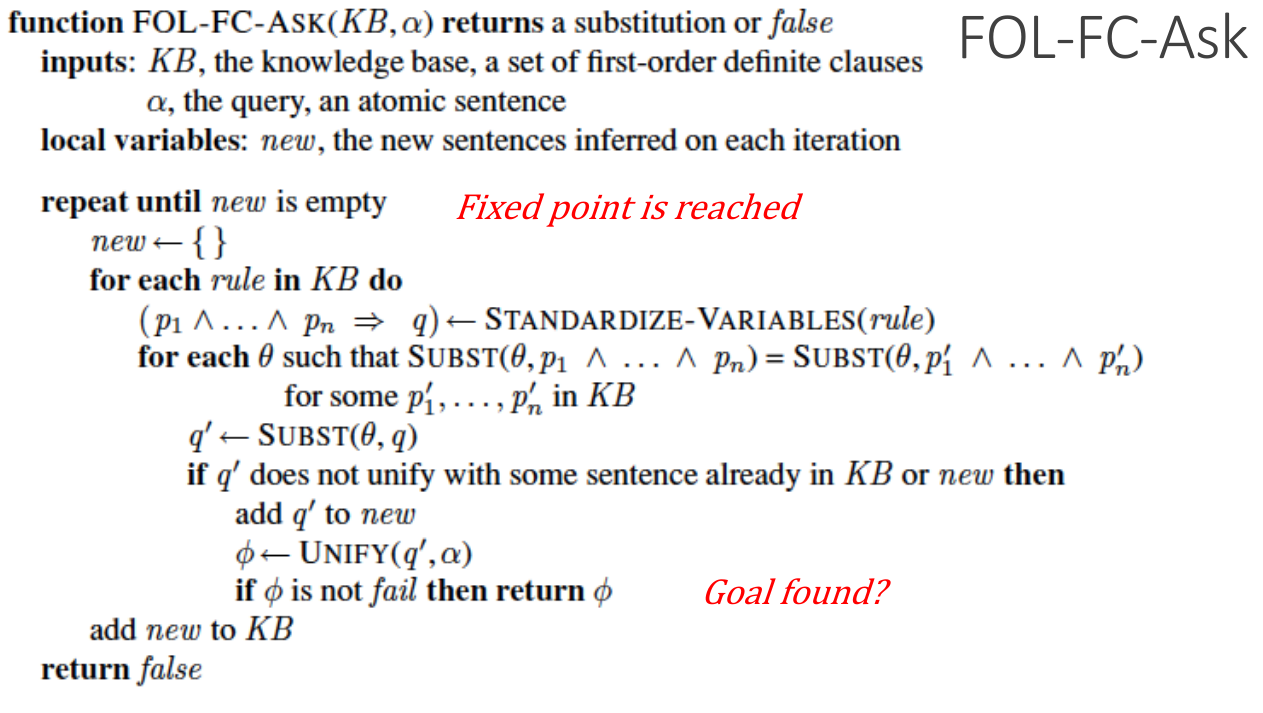
\includegraphics[width=\textwidth]{Images/forwardChaining}
	\caption{Pseudocode for Forward chaining}
	\label{img:forwardChaining}
\end{figure}
In figure \ref{img:forwardChaining} is possible to note the pseudocode for Forward chaining
and the interpreter is required to perform many unification operations, so if we have
$r$ rules to try (in OR), $n$ preconditions in each rules to be satisfied (in AND) and 
$w$ facts in the KB (in OR) and everything repeated for c cycles so we have 
$r \times n \times w \times c$ unification operations.

Finding all the facts that unify with a given pattern can be made more efficient 
with appropriate predicate indexing, so a hash table on the head of the predicate,
in the simplest case, but in complex case we can use a hash table with a combined key head
$+$ first argument and/or a discrimination network on the antecedents of the rules.\newline
Another improvents is that each rule does not need to be checked again at each iteration, so
only the ones which are affected by recent additions.
This two strategies are among the strategies implemented by the RETE algorithm included
in Production Systems and rule-based programming languages such as CLIPS.

Another improvement is the \emph{Conjunct ordering}, which the order in which you list
antecedents of rules is important for efficiency.\newline
Each antecedent is a constraint and each rule a CSP, so we can apply heuristics from CSP for
ordering and we can try to write rules which correspond to CSP with a tree-structure.\newline
The last improvement is that proceeding forward may lead to derive many irrelevant facts,
so we restrict the forward chaining to the relevant rules for the goal by proceeding backward
and marking them (in deductive databases are called \emph{Magic sets}).

Rule-based systems are one of the first paradigms for representing knowledge in A.I. and 
most expert systems are rule-based.\newline
Rules are used forward to produce new facts, hence the names productions and production systems
and they are a general computational model based guided by patterns: the rule to be applied
next is determined by the operation of pattern matching, a simplified form of unification.

CLIPS (C Language Integrated Production System”) is a successor of OPS-5 (Forgy), 
developed by NASA and now freely available at \href{http://www.clipsrules.net/}.

A typical rule-based system has four basic components:
\begin{enumerate}
   \item A list of facts (no variables), the temporary \emph{Working Memory} (WM), defined as 
	   \begin{lstlisting}
	   (predicate arg_1 arg_2 \dots arg_k) %ordered facts 
	   (predicate (slot_1 val_1) \dots (slot_k val_k)) %structured facts}
	   \end{lstlisting}
   \item A list of rules or rule base, a specific type of knowledge base, represented as 
	   \begin{lstlisting}
	      (defrule rule\_name ["comment"] 
		(pattern_1) (pattern_2) \dots (pattern_k) \Rightarrow (action_1) (action_2) 
		\dots (action_m) 
	   \end{lstlisting}
   \item An interpreter, called \emph{inference engine}, which infers new facts or takes action
	 based on the interaction of the WM and the rule base.
   \item A conflict resolution strategy.
\end{enumerate}
The interpreter executes a match-resolve-act cycle, which consist to 
\begin{description}
   \item [Match: ] the Left-Hand-Sides (LHS) of all rules are matched against the contents
	   of the working memory and this produces a conflict set: instantiations
           of all the rules that are satisfied/applicable.
   \item [Conflict-Resolution: ] one of the rules instantiations in the conflict set is
          chosen for execution and if no applicable rule, the interpreter halts.
   \item [Act: ] the actions in the Right-Hand-Side (RHS) of the rule selected in the
          conflict-resolution phase are executed and these actions may change the
          contents of working memory and this cycle repeats.
\end{description}
Matching rules (activations) are put in an agenda from where one will be selected and 
newly activated rules are added to the agenda and the agenda is reordered
according to the salience of the rules.\newline
Among the rules of equal salience, the current conflict resolution strategy is used
to determine the rule to be fired (analogy with neurons) and the depth strategy is the 
standard default strategy of CLIPS (new rules on top).\newline
Different predefined conflict resolution strategies under user control:
\begin{description}
   \item [breadth: ] newly activated rules are placed below all rules of the same salience.
   \item [simplicity: ] among rules of the same salience, less specific rules are preferred.
   \item [complexity: ] among rules of the same salience, most specific rules are preferred.
   \item [random: ] among rules of the same salience, choose at random and this is 
	           useful for debugging.
\end{description}
The advantages of production systems are that writing rules is very natural for experts or 
end-users, justification of conclusions is possible and it is a general programming paradigm,
which can be extensible with user defined functions and OOP for object definition.\newline
Disadvantages are that it may be difficult to control the firing of rules and expressing
knowledge as rules may be a bottleneck.

We consider now backward chaining and we start from SLD resolution, where 
a SLD derivation of a clause $c$ from $KB$ is a sequence $S$ of clauses
$c_1, c_2, \dots, c_n$ such that $c_1 \in KB, c_n = c$ and each $c_{i+1}$ is obtained 
by the resolution rule applied to $c_i$ and some clause in $KB$.\newline
In backward reasoning systems the SLD strategy is used by refutation, so we starting from the
negation of the goal and trying to derive the empty clause.\newline
The SLD strategy is complete for Horn clauses, so $KB \models c \Rightarrow S \vdash_{SLD} c$
and propositional Horn clauses KB's have linear-time deduction algorithms.

A logic program is a set of definite Horn clauses (facts and rules), so for example
\[ A. \]
\[ A:- B_1, B_2, \dots, B_n. \]
The declarative interpretation of this example is that $A$ is true and $B_1, B_2, \dots, B_n
\Rightarrow A$.\newline
The goal is a negative clause, written as $?- G_1, G_2, \dots, G_k$ (a conjunction of subgoals).

The procedural interpretation is that the head of a rule can be seen as a function call
and the body as functions to be called in sequence, so when they all return
the main procedure returns.

Given a logic program and a goal $G_1, G_2, \dots, G_k$ the SLD goal tree is constructed
as follows: each node of the tree corresponds to a conjunctive goal to be solved.\newline
The root node is $?- G_1, G_2, \dots, G_k$, let $?- G_1, G_2, \dots, G_k$ a node in the tree
and the node successors are obtained by considering the facts and rules in the program
whose head unifies with $G_1$.\newline
If $A$ is a fact and $\gamma = MGU(A, G_1)$, a descendent is the new goal
$?- (G_2, \dots, G_k)\gamma$, instead if $A :- B_1, \dots, B_m$ is a rule and 
$\gamma = MGU(A, G_1)$, a descendent is the new goal 
$?- (B_1, \dots, B_m, G_2, \dots, G_k)\gamma$.
Note that variables in rules are renamed before using them, nodes that correspond
to empty clauses are successes and nodes without successors are failures.

\begin{figure}
	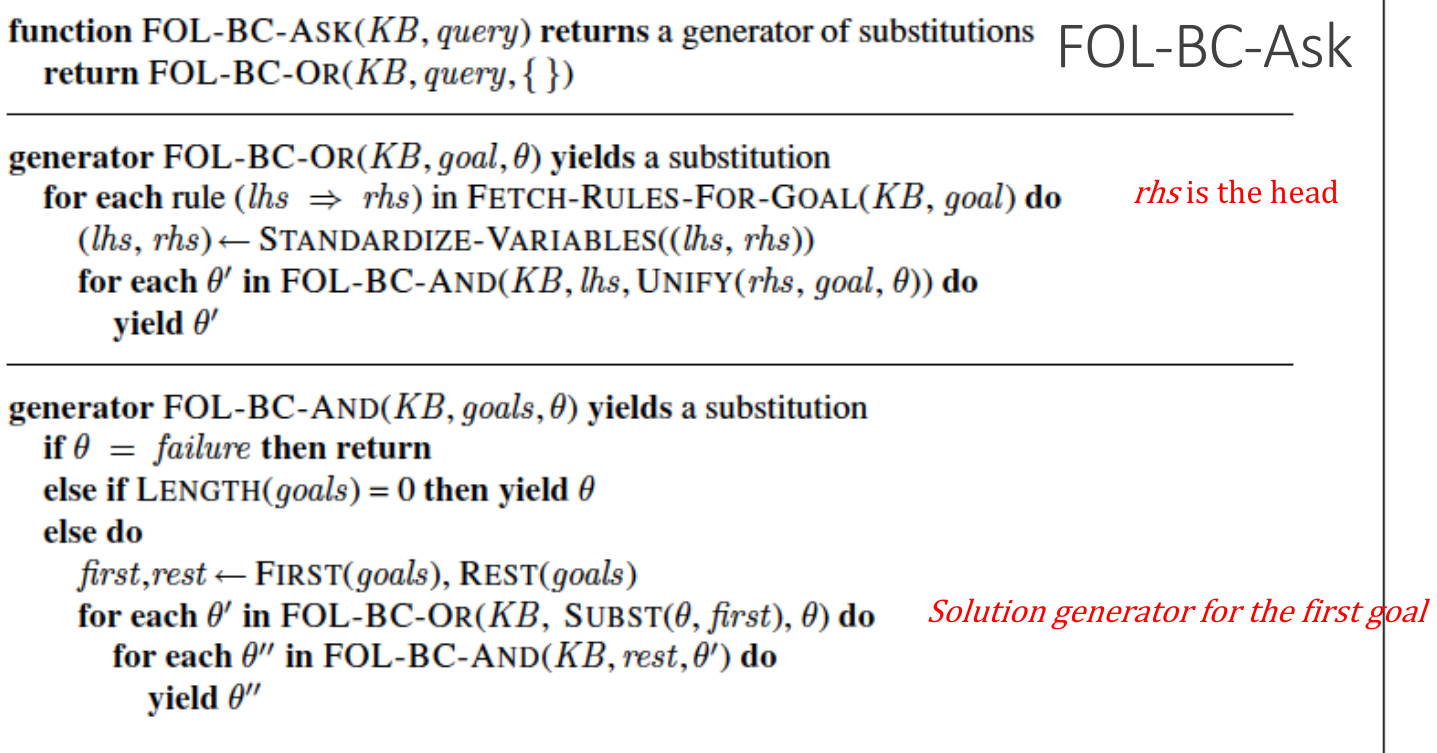
\includegraphics[width=\textwidth]{Images/sldPseudo}
	\caption{Pseudocode for SLD resolution strategy}
	\label{img:backward}
\end{figure}
The SLD resolution strategy is complete for definite Horn clauses, with pseudocode visible
in figure \ref{img:backward}, so this means that if $P \cup \{\neg G \}$ is unsatisfiable,
then at least one of the leaves of the SLD tree produces the empty clause (success).\newline
Moreover trying to satisfy the subgoals in the order they appear it is not
restrictive, since in the end all of them must be satisfied and when there are variables
in the goal, the substitution that we obtain is the computed answer.\newline
Completeness and efficiency are however influenced by the order of expansion of the nodes
(the visit strategy of the SLD tree), the order in which we consider successor nodes at
each level and the order of literals in the body.

Observations arrive online from the user or from sensors and we cannot expect users or
sensors to provide all relevant information.\newline
The solution is to introduce an “ask-the-user” mechanism into the backward procedure, so 
define askable atoms: those atom for which the user is expected to provide 
an answer when unknown.\newline
In the top-down procedure if the system is not able to prove an atom,
and the atom is askable, it asks the user.

Explanations are required and a strong pro of rule-based decision support systems wrt
other AI techniques, so support can be provided for three different kinds of requests:
\begin{enumerate}
   \item How questions: how a fact was proved.
   \item Why questions: why the system is asking about this?
   \item Whynot questions: why a fact was not proved?
\end{enumerate}
Given that the inference engine is correct, misbehaviors can only be caused by faulty
knowledge, and debugging can be done by the domain expert, provided he/she is aware of 
the meaning of symbols.\newline
Four types of errors can be supported in debugging:
\begin{enumerate}
   \item Incorrect answers
   \item Missing answers
   \item Infinite loops
   \item Irrelevant questions
\end{enumerate}
We need an extension of the language to deal with integrity constraints of this form
\[ F \gets a_1 \land \dots a_k \equiv \not a_1 \lor \dots \not a_k \]
We have that a Definite Horn database is always satisfiable and a Horn database
(including integrity constraints) can be unsatisfiable.\newline
Discovering a contradiction in the KB can be important in many applications and for these
tasks you must declare a set of assumables, atoms that can be assumed 
in a proof by contradiction.\newline
The system can then collect all the assumable that are used in proving false and that is
\[ KB \cup \{c_1, \dots, c_r\} \models F \]
where $C = \{c_1, \dots, c_r\}$ is a conflict of KB and a possible answer is 
\[ KB \models \not c_1 \lor \dots \lor \not c_r \]
A \emph{minimal conflict} is a conflict such that no strict subset is also a conflict.

The aim of consistency-based diagnosis is to determine the possible faults based on a model
of the system and observations of the system.\newline
Background knowledge provides the model of the system, we make the absence of faults assumable,
conflicts with observations can be used to derive what is wrong with the system and in the end
from set of conflicts we can derive a minimal diagnosis.\newline
A consistency-based diagnosis is a set of assumables that has at least one element 
in each conflict and a minimal diagnosis is such that no subset is a diagnosis.

We have $a \iff b_1 \lor \dots \lor b_n$, that is the \emph{Clark's completion}, and under 
Clark's completion if there are no rules for $a$ then $a$ is false.\newline
With this, the system is able to derive negations, so we extend the language of definite
Horn clauses with not and note that this negation is not the same as logical $\not$,
so we use a different notation.\newline
In backward reasoning systems this not can be implemented by negation as failure.

The top-down procedure for negation as failure is defined as follows: not p can be
added to the set of consequences whenever proving $p$ fails.\newline
The failure must occur in finite time, there is no conclusion if the proof procedure does
not halt and \emph{Negation as failure} is the same as a proof of a logical negation
from the KB under Clark's completion $KB_c$, so formally is 
\[ KB_c \models \not a \text{ iff } KB \not \vdash a \]
Negation as failure is a form of non-monotonic reasoning, so we can express defaults.

\emph{Abduction} is a form of reasoning which consists in providing explanations for
observations and the term abduction was coined by Peirce ($1839$–$1914$) to differentiate
this type of reasoning from deduction, which involves determining what logically follows from
a set of axioms, and induction, which involves inferring general relationships from examples.

Given a knowledge base $KB$, which is a set of of Horn clauses, a set $A$ of assumable atoms,
the building blocks of hypotheses.\newline
An explanation of $g$ is a set $H$ such that $H \subseteq A$ such that
$KB \cup H \not \models F$ and $KB \cup H \models g$ and we usually want a 
minimal explanation, since there can be more than one explanation.

Abductive diagnosis, provides explanation of symptoms in terms of diseases or malfunctions,
so both the normal and the faulty behavior need to be modelled in order to infer observations 
and observations are not added to the KB.\newline
Consistency based diagnosis needs only to represent normal behavior and observations are
added to the KB to obtain inconsistencies and abductive diagnosis requires
more detailed models, allowing to derive faulty behavior as well.

\section{Prolog}
Prolog is the most widely used logic programming language and we have already introduced 
the syntax and the execution model (SLD resolution).\newline
The declarative semantics is given by Horn clause knowledge bases and the procedural semantics
is given by a specific strategy for exploring SLD trees, successors are generated in the 
order they appear in the logic program and the SLD tree is generated left-to-right depth first,
also in the end the occur check is omitted from PROLOG's unification algorithms, so as a 
consequence Prolog is not complete and also is not correct.

Prolog uses the database semantics rather than first-order semantics, so it has unique name 
and closed word assumption (a form of nonmonotonic reasoning like negation as failure).\newline
Prolog is a full-fledged programming language, since has an efficient implementation of the 
interpreter, there are built-in functions for arithmetic and list manipulation.

A Prolog interpreter is similar to Forward Chaining ask algorithm but is more efficient, since
rely on a global data structure, a stacj of choice points.\newline
Logic variables in a path remember their bindings in a trail and when failure occurs, the 
interpreter backtracks to a previous choice point and undoes the bindings of the variables.

Prolog compiles into an intermediate abstract machine (the Warren abstract Machine) and 
parallelism cna be exploited by OR-parallelism or AND-parallelism.

In forward chaining we do not have the problem of repeated computation, and we can obtain a 
similar saving in backward systems with a technique called \emph{memoization}, which consists
in caching solutions to subgoals and reusing them.\newline
Tabled logic programming systems use efficient storage and retrieval mechanisms to 
perform memoization.

Basic data types in Prolog are numbers, atoms (identifiers with initial lowecase) and 
Variables (identifiers with initial uppercase and anonymous variables use $\_$).\newline
Structured objects are functions with arguments (functor applied to arguments), like 
$date(1, may, 2001)$ and lists, like for example $[ann, john, tom, alice]$.

We have as basic arithmetic operations $+, -, *, /, //, **, mod$ and so on, where 
$//$ is the integer division.\newline
The $is$ infix operator forces the evaluation of the expressions and we use as comparison
operators 
\begin{lstlisting}[language=Prolog]
<, >, <=, >=, =:=, =\=
\end{lstlisting}
where the last two are the equal and not equal operators which force evaluation.

To improve performance of Prolog programs it is better that programmers choose the order
of clauses and subgoals that require less nodes to consider.\newline
Prolog will automatically backtrack if this is necessary to satisfy a goal and uncontrolled 
backtracking however may cause inefficiency in a Prolog program so we introduce cut $!$, 
so $G:-T, !, R.$ and $G:-S.$ will execute S if $T$ is not true otherwise we will execute $R$.

The negation as failure is implemented in Prolog using the built-in procedure not, that fails
if $P$ succeeds otherwise fails and failure must occur in a finite number of steps.

Using cut has advantages and drawbacks, with cut we can often improve the efficiency of the 
program and the idea is to explicitly tell Prolog to do not try other alternatives because
they are bound to fail.\newline
Using cut we can specify mutually exclusive rules, so we can add expressivity to the language.

The main disadvantage is that we can lose the correspondence between the declarative and 
procedural menaning of programs and two kinds of cut can be distinguished:
\begin{description}
   \item [Green cuts: ] that do not change the meaning (safe).
   \item [Red cuts: ] that change the meaning, we have to be careful to the actual meaning.
\end{description}

Constraint logic programming (CLP) combines the constraint satisfaction approach with 
logic programming, creating a new language where a logic program works along a specialized
constraint solver.\newline
The basic Prolog can be seen as a very specific constraint satisfaction language where 
the constraints are of a limited form, that is equality of terms 
(unifications constraints or bindings).\newline
Prolog is extended introducing other types of constraints and $CLP(X)$ differ 
in the domain and type of constraints they can handle, so for example $CLP(R)$ handles 
constraints on real numbers, $CLP(Z)$ for integers, $CLP(Q)$ is for rational numbers,
$CLP(B)$ for boolean values and $CLP(FD)$ are for finite domains.

A CLP solution is the most specific set of constraintson the variables that can be derived
from the knowledge base and is a specific solution if the constraints are tight enough.\newline
In figure \ref{img:constraintsProlog} is possible to compare the behavior a classical Prolog
program with a CLP program.

\begin{figure}
	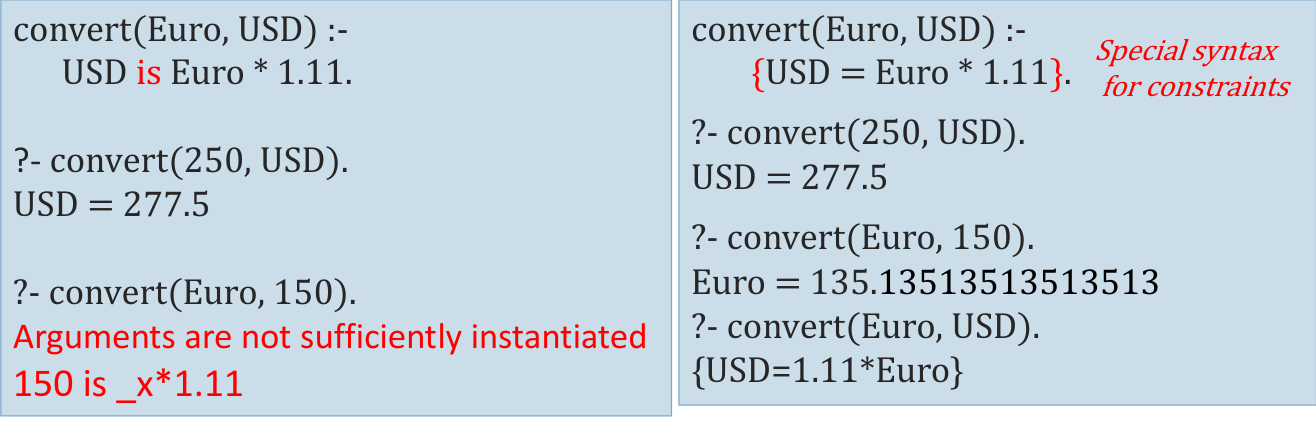
\includegraphics[width=\textwidth]{Images/constraintsProlog}
	\caption{Comparison between Prolog and CLP program}
	\label{img:constraintsProlog}
\end{figure}
A meta-interpreter for a language is an interpreter that is written in the language itself and
Prolog has a powerful features for writing meta programs because Prolog treats programs
and data both as terms.\newline
A program can be input to another program and also one can write meta interpreters 
for various applications, extending the implementation of Prolog in different directions.\newline
Applications is exploring different execution strategies for the interpreter, like 
on breadth first, limited depth search, combination of depth-first and breadth-first searches and
so on.\newline
It is also possible generating proof trees and implementing new languages and/or an OOP 
implementation in Prolog.\newline
To build the meta-interpreter we can rely on the built-in predicate $clause(Goal, Body)$ and 
given a program and a goal, it retrieves a clause from the consulted program that matches 
Goal and Body then can be executed and in figure \ref{img:interpreter} is visible an 
interpreter implementation done using Prolog.

\begin{figure}
	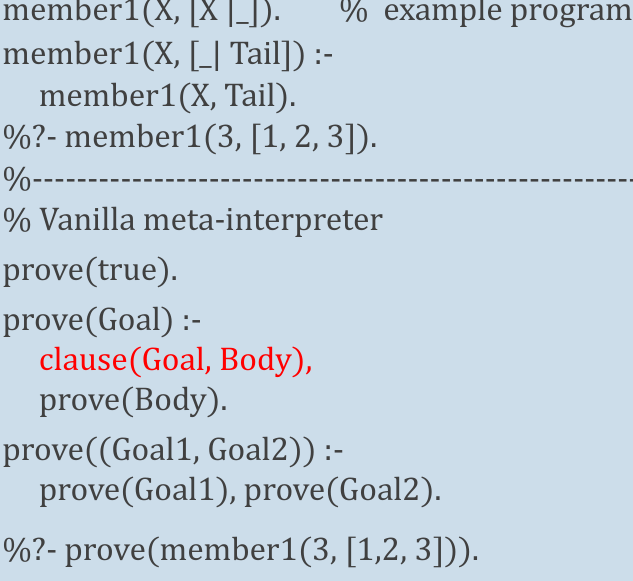
\includegraphics[width=\textwidth]{Images/metaInterpreter}
	\caption{Meta interpreter implementation with Prolog}
	\label{img:interpreter}
\end{figure}

\section{Answer Set Programming}
Answer Set programming/Prolog is a language for KR\&R based on the stable model semantics of
logic programs (an alternative, more declarative, semantics) and it includes, in a coherent
framework, ideas from declarative programming, expressive KR language, deductive databases
(forward reasoning), but also disjunctive databases; it includes also
syntax and semantics of standard Prolog as a special case 
(but also disjunction, "classical" and "strong" negation, constraints) and from
nonmonotonic logic (defaults, preference models, autoepistemic logic).\newline
Useful real world applications are team building, bio-informatics, linguistics, but are 
not exhaustive since there are several real world applications.

\begin{figure}
	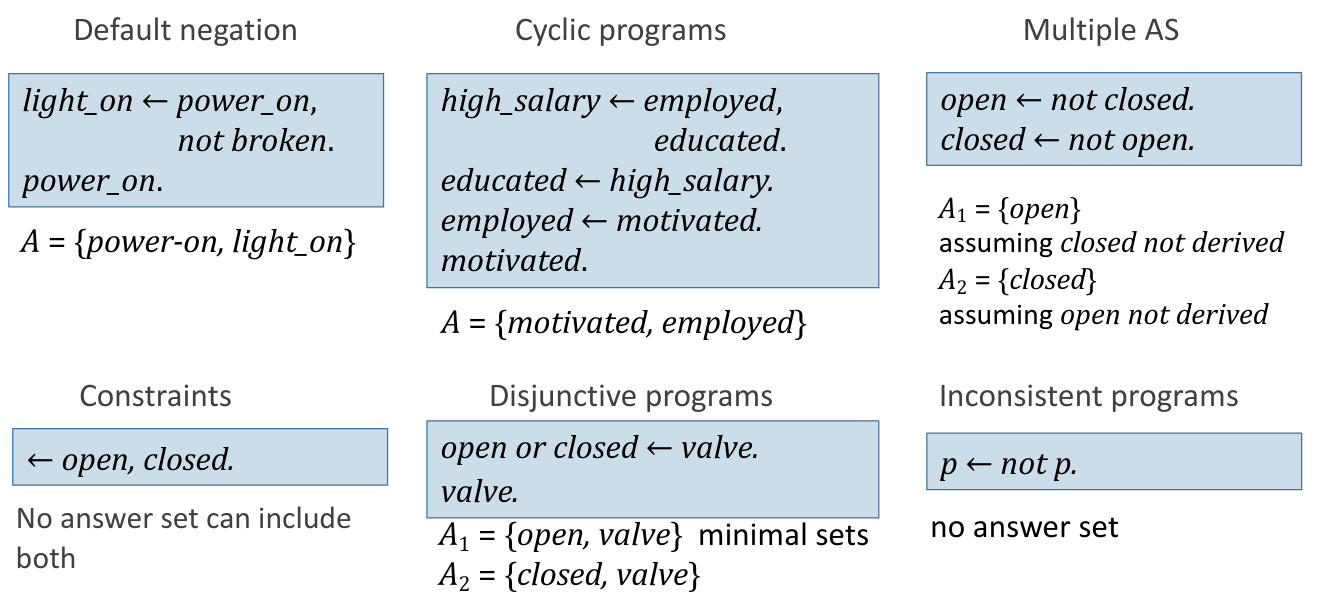
\includegraphics[width=\textwidth]{Images/answerSet}
	\caption{Example of Answer Set}
	\label{img:answerSets}
\end{figure}
Answer sets are sets of beliefs (AS) that can be justified on the basis of the program, 
as we can see in figure \ref{img:answerSets}, and we assume sorted signatures from 
classic logic, including natural numbers and arithmetic operators.\newline
Literals are $p(t)$ and $\neg p(t)$ where $t$ are sequences of terms and 
a rule is an expression of the form 
\[ l_0 \lor \dots \lor l_k \gets l_{k+1}, \dots, l_m, \neg l_{m+1}, \dots, \neg l_n. \]
where the head is all terms before $\gets$, the body are all terms after $\gets$.

Programs without $\neg$(the strong negation) and without or ($k = 0$) are called 
\emph{normal logic programs} (nlp).\newline
When  $head(r) = \{ \}$ the rule is called a \emph{constraint} and when $body(r) = \{\}$
the rule is called a \emph{fact}.

A program of Answer Set Prolog/Programming is a pair $\{\sigma, Pi\}$ where $\sigma$ is a
signature and $\Pi$ is a collection of logic programming rules over $\sigma$.\newline
The signature $\sigma$ is defined by the following rules:
\begin{itemize}
    \item Sorts/constants $\tau_1 = \{a, b\}$ and $\tau_2 = N$ where $N = \{0, 1, \dots\}$.
    \item Predicates $p(\tau_1), q(\tau_1, \tau_2), r(\tau_1)$ and the standard relation
	  $<$ on $N$.
\end{itemize}
Note that the signature may be derived from the program, $\sigma(\Pi)$, rather than being
given explicitly and it consist of all the constants which appear in the program.\newline
Terms, literals, and rules are called ground if they contain no variables and no symbols
for arithmetic functions and we define the following concepts:
\begin{description}
    \item [Herbrand universe: ] the set of all ground istances of terms.
    \item [Herbrand base: ] the set of all ground atomic sentences.
\end{description}
A program $gr(\Pi)$ consisting of all ground instances of all rules of $\Pi$ 
is called the \emph{ground instantiation} of $\Pi$.\newline
In figure \ref{img:groundProgram} is possible to note an example of Answer program and 
the relative ground instances.
\begin{figure}
	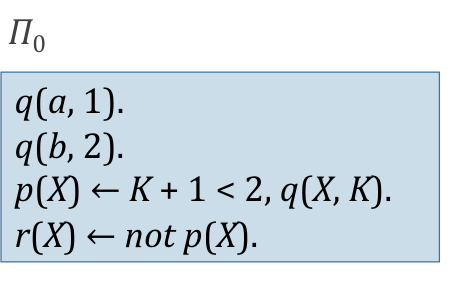
\includegraphics[width=0.45\textwidth]{Images/exampleAnswer}
	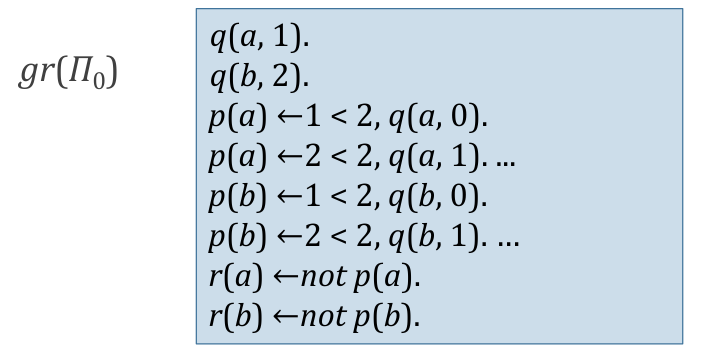
\includegraphics[width=0.45\textwidth]{Images/exampleGround}
	\caption{Example of Ground program}
	\label{img:groundProgram}
\end{figure}

A (partial) interpretation is a consistent subset of the Herbrand base and a partial
interpretation $S$ is a consistent set of ground literals over $\sigma$.
Given two contrary literals $l$ and $l^-$, $l$ is true if $l \in S$ and $l$ is false if 
$l^- \in S$, otherwise $l$ is unknown in $S$.\newline
An extended literal $not l$ is true in $S$ if $l \not \in S$ otherwise $not l$ is false
in $S$; a set of extended literals $U$, represented as conjuction is true if all of them
are true and is false if at least one is false otherwise is unknown.\newline
A disjunction of literals $\{l_0 or \dots or l_k\}$ is true if at least one is true, false 
if all of them are false in $S$ otherwise is unknown.\newline
We have that $S$ satisfies a rule $r$ if $S$ satisfies $r$'s head or does not satisfy its body.

The answer set semantics of a logic program $\Pi$ assigns to $\Pi$ a collection 
of answer sets $S$ and an answer set is a partial interpretations over $\sigma(\Pi)$
corresponding to possible sets of beliefs which can be built by a rational reasoner
on the basis of rules of $\Pi$.\newline
Each answer set $S$ obeys the following principles:
\begin{description}
   \item [Consistency: ] $S$ must satisfy the rules of $\Pi$.
   \item [Minimality: ] a rationality principle, "do not believe anything you are not
	                forced to believe".
\end{description}

\begin{figure}
	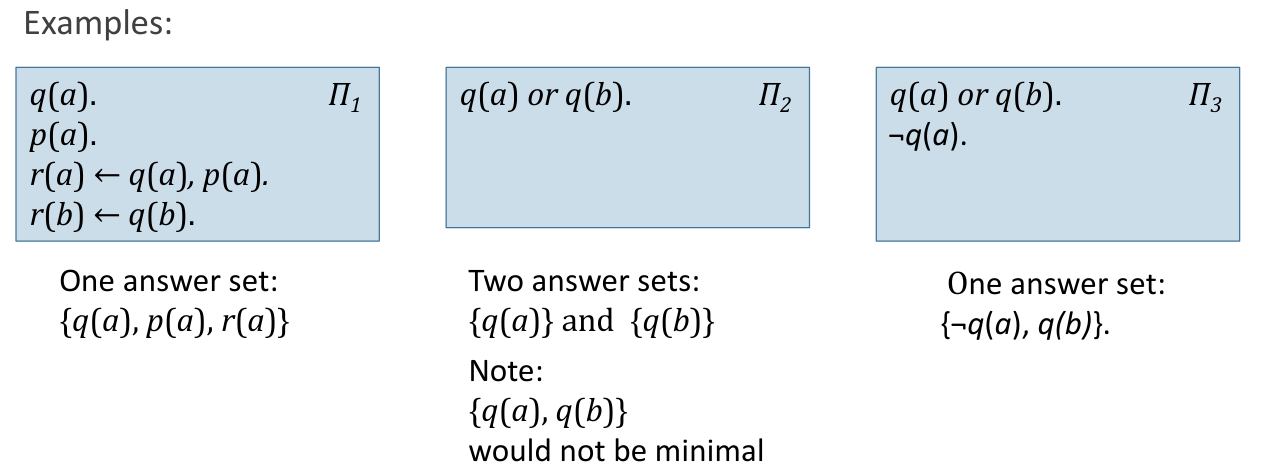
\includegraphics[width=\textwidth]{Images/answerSetNotNegative}
	\caption{Example of Answer Set without default negative}
	\label{img:answerSetNotNegative}
\end{figure}
\begin{figure}
	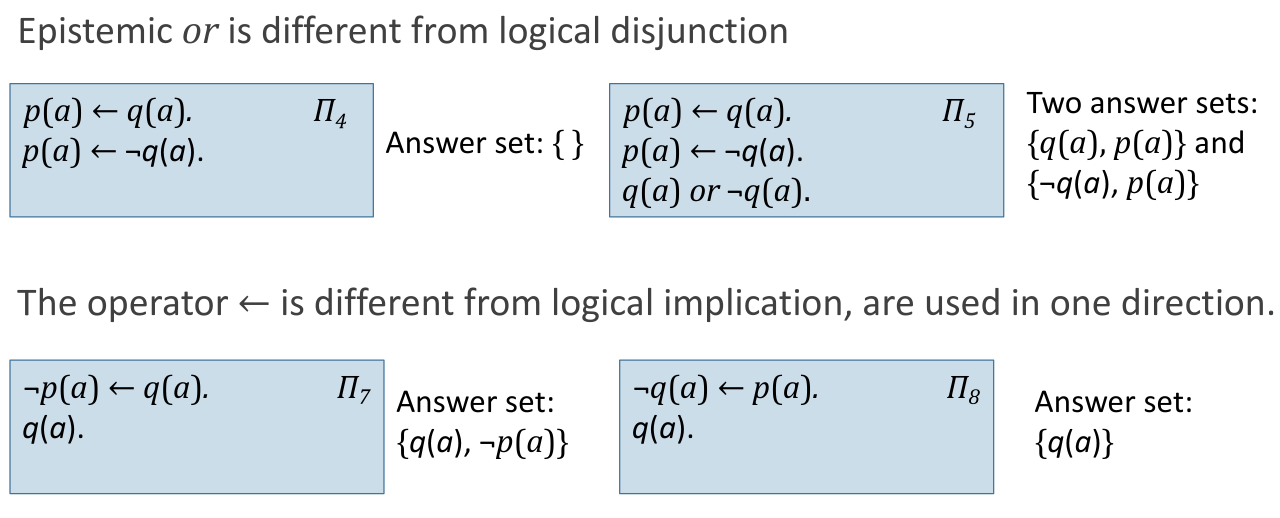
\includegraphics[width=\textwidth]{Images/answerSetMoreEx}
	\caption{Another Example of Answer Set without negative}
	\label{img:answerSetMoreEx}
\end{figure}
A partial interpretation $S$ of $\sigma(\Pi)$ is an answer set for $\Pi$ if $S$ is
minimal (in the sense of set-theoretic inclusion) among the partial interpretations
satisfying the rules of $\Pi$.\newline
Epistemic or is different from logical disjunction and also the operator $\gets$ is different
from logical implication, since are used in one direction.\newline
In figure \ref{img:answerSetNoNegative} and \ref{img:answerSetMoreEx} are possible to note
some example about answer set in program without default negative.\newline
To consider also default negative the approach consist to generate answer sets, simplify 
rules and check.\newline
Reduct $\Pi^S$ of $\Pi$ wrt a partial interpretation $S$ is the set of rules 
obtained from $\Pi$ consist to dropping every rule 
$A \gets B_1, \dots, B_m, not C_1, \dots, not C_n$ such that at least one of the negated 
atoms $C_i$ in its body belongs to $S$ (rule is not applicable) and also 
dropping $not C_j$ from the body of the rules when $C_j$ does not belong to $S$
(condition is satisfied).\newline
A partial interpretation $S$ of $\sigma(\Pi)$ is an answer set for $\Pi$ if $S$ 
is an answer set for $\Pi^S$ , the reduct of $\Pi$, as defined before.

A program $\Pi$ entails a ground literal $l$ $(\Pi \models l$) if $l$ is satisfied by 
every answer set of $\Pi$ and we say that the program $\Pi$'s answer to a query $q$ is
yes if $\Pi \models q$, no if $\Pi \models \not q$ and unknown otherwise.

A logic program is called consistent if it has an answer set and inconsistencies may be due
to improper use of logical negation.\newline
We can transform a ASP program $\Pi$ to one without negation $\Pi^+$ (the positive form)
and the transformation works as follows:
\begin{enumerate}
   \item for each predicate symbol $p$ we introduce a symbol $p'$ with the same arity.
   \item we replace each $l = \not p(t)$ with $p'(t)$, its positive form, $l^+$ and if $l$
	 is positive we set $l = l^+$.
\end{enumerate}
A logic program $\Pi$ can be transformed in its positive form $\Pi^+$ by replacing each rule with
\[ \{l_0^+, \dots, l_k^+\} \gets l_{k+1}^+, \dots l_m^+, not l_{m+1}^+, \dots, not l_n^+ \]
and adding the constraints $\gets p(t), p'(t)$ for each $p'$ added.\newline
A property is that a set $S$ of literals of $\sigma(\Pi)$ is an answer set of $\Pi$ 
iff $S^+$ is an answer set of $\Pi^+$.

A logic program can be inconsistent for the use of the default negation and in general
the problem of checking consistency is undecidable or decidable and very complex for
finite domains.\newline
The theory helps us in making simplifying assumptions to guarantee consistency, so we define
\begin{defi}[Level Mapping]
A function $||.||$ which maps ground atoms in $P$ (the Herbrand base of $P$) to natural
numbers and if $D$ is a disjunction or conjunction of literals, $||D||$ is defined as the
minimum level of atoms occurring in literals from $D'$ (the positive form).\newline
This also implies that $||\not l|| = ||l||$.
\end{defi}
\begin{defi}[Locally stratified program]
A logic program $\Pi$ is locally stratified if it does not contain $\not$,
and there is a level mapping of the grounded version of $\Pi, gr(\Pi)$ such that for
every rule:
	\[ \forall l \in pos(r) \, ||l|| \leq ||head(r)|| \]
	\[ \forall l \in neg(r) \, ||l|| < ||head(r)|| \]
\end{defi}
\begin{defi}
   If a program is locally stratified and, in addition, for any predicate symbol $p$,
   $||p(t_1 )|| = ||p(t_2 )||$ for any $t_1$ and $t_2$, the program is called stratified.
\end{defi}
A stratified program is also locally stratified and a program without not is stratified.

Properties are the following:
\begin{enumerate}
   \item A locally stratified program is consistent.
   \item A locally stratified program without disjunction has exactly one answer set.
   \item The above conditions hold by adding to a locally stratified programs a collection
	 of closed world assumptions of the form $\not p(X) \gets not p(X)$.
\end{enumerate}
There are weaker syntactic conditions that still guarantee consistency, 
for example order-consistent programs.

The choice of the algorithms used depend on the structure of problems and the type of
queries, so we consider for example Normal logic programming acyclic programs 
and Tight programs.
\begin{defi}[Acyclic programs]
A normal logic program $\Pi$ is called acyclic if there is a level mapping of $\Pi$ such that
for every rule $r$ of $gr(\Pi)$ and every literal $l$ which occurs in $pos(r)$ or $neg(r)$,
$||l || < ||head(r)||$
\end{defi}
If $\Pi$ is acyclic then the unique answer set of $\Pi$ is the unique Herbrand/classical model
of Clark’s completion of $\Pi, Comp(\Pi)$.\newline
SLDNF resolution-based interpreter of Prolog will always terminate on atomic queries
and produce the intended answers.

\begin{defi}[Tight programs]
A normal logic program $\Pi$ is called tight if there is a level mapping of $\Pi$ such that
for every rule $r$ of $gr(\Pi)$ and every literal $l \in pos(r), head(r) > l$.
\end{defi}
Acyclic programs are tight but no vice versa and if program $\Pi$ is tight then answer sets
of $\Pi$ are the models of the Clark’s completion of $\Pi$.\newline
The problem of computing answer sets can be reduced to SAT for propositional formulas
and a SAT solver can be used and also in the case of not tight programs there are 
theoretical results that allow translating into SAT problems, even if very large.

These theoretical results have led to the development of answer set solvers such as ASET,
CMODELS, and so on, which are based on (possibly multiple) calls to propositional solvers.

Traditional answer set (AS) solvers typically have a two level architecture:
\begin{description}
   \item [Grounding step: ] compute $gr(P)$ and grounders can be integrated (e.g. DLV)
	                    or provided as separate modules.\newline
           The size of the grounding (even if partial) is a major bottleneck and 
	   smart and lazy grounding techniques have been developed.
   \item [Model search: ] the answer sets of the grounded (propositional) program are computed.
\end{description}
The workflow of Answer Set programming is possible to note in figure \ref{img:answerSolver} and
applications are in repairing large scale biological networks, planning, decision making
but also Industrial integration and Music composition system.

\begin{figure}
	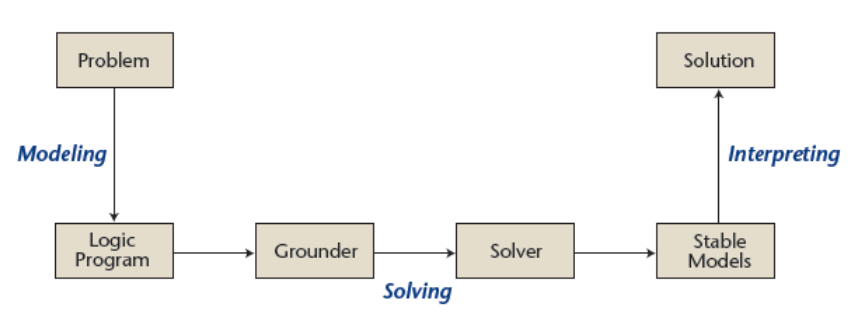
\includegraphics[width=\textwidth]{Images/answerSolver}
	\caption{Workflow of Answer Set programming}
	\label{img:answerSolver}
\end{figure}
